\bgroup  
\begin{frame}{Likelyhood $P(X/Y)$}
\textbf{Naive assumption}: all pixels are independent given the class. The probability of an image is the product of the probability of every single pixel.\\
\begin{equation*}
P(X_i/Y_c)=\prod_{j=1}^m P(x_i^{(j)}/Y_c)
\end{equation*}
During training, we need to model this for each possible class:
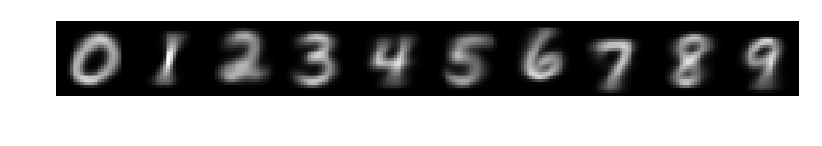
\includegraphics[width=\textwidth]{img/lkl_model.pdf}
\end{frame}
\egroup